\documentclass{standalone}
\usepackage{tikz}
\usetikzlibrary{arrows.meta}
\begin{document}
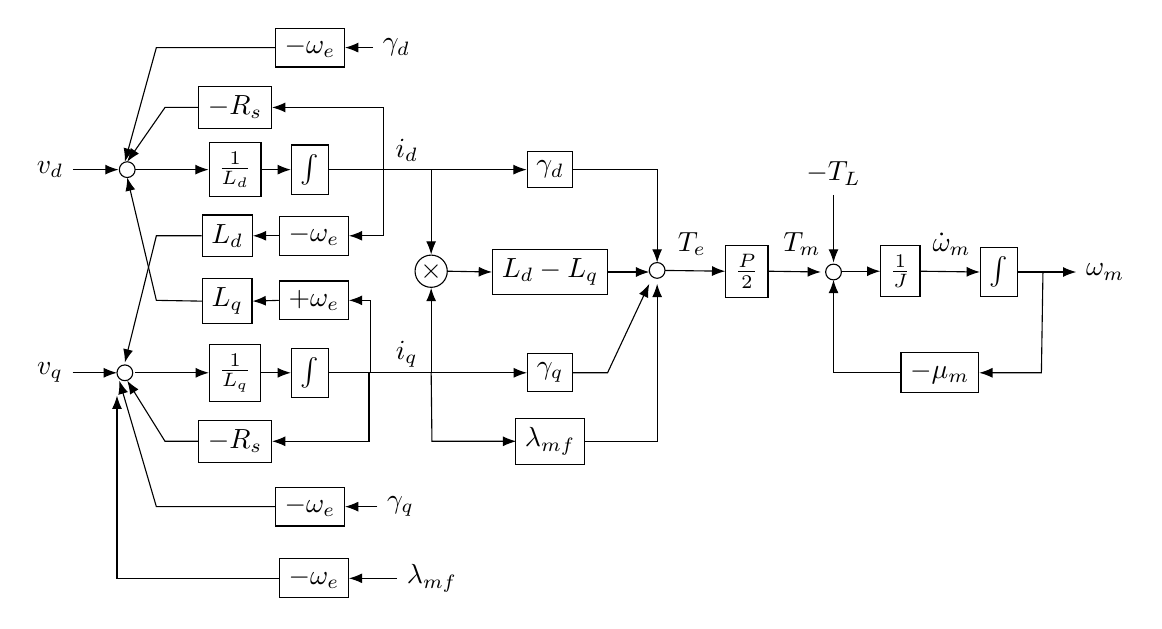
\begin{tikzpicture}
  \node (node1) at (-0.35,2.45) {$v_d$};
  \draw[arrows=-Latex] (node1.east) -- (0.52,2.45);
  \draw (0.63,2.45) circle (0.1cm);
  \node[draw] (node2) at (2.95,2.45) {$\int$};
  \node[draw] (node3) at (2,3.24) {$ -R_s$};
  \draw[arrows=-Latex] (node3.west) -- (1.11,3.24) -- (0.63,2.55);
  \draw[arrows=-Latex] (3.88,2.4) -- (3.88,3.24) -- (node3.east);
  \node (node4) at (-0.35,-0.13) {$v_q$};
  \node[draw] (node5) at (2.95,-0.13) {$\int$};
  \draw[arrows=-Latex] (node4.east) -- (0.5,-0.13);
  \draw (0.6,-0.13) circle (0.1cm);
  \node[draw] (node3) at (2,-1) {$ -R_s$};
  \draw[arrows=-Latex] (node3.west) -- (1.11,-1) -- (0.63,-0.23);
  \draw[arrows=-Latex] (3.7,-0.13) -- (3.7,-1) -- (node3.east);
  \node[draw] (node10) at (2,2.45) {$\frac{1}{L_d}$};
  \draw[arrows=-Latex] (0.73,2.45) -- (node10.west);
  \node[draw] (node11) at (2,-0.13) {$\frac{1}{L_q}$};
  \node[draw] (node7) at (1.9,1.61) {$L_d$};
  \node[draw] (node6) at (1.9,0.78) {$L_q$};
  \node[draw] (node8) at (3,1.61) {$-\omega_e$};
  \node[draw] (node9) at (3,0.79) {$+\omega_e$};
  \draw[arrows=-Latex] (3.72,-0.13) -- (3.72,0.79) -- (node9.east);
  \draw[arrows=-Latex] (3.88,2.45) -- (3.88,1.61) -- (node8.east);
  \draw[arrows=-Latex] (node8.west) -- (node7.east);
  \draw[arrows=-Latex] (node9.west) -- (node6.east);
  \draw[arrows=-Latex] (node10.east) -- (node2.west);
  \draw[arrows=-Latex] (node11.east) -- (node5.west);
  \draw[arrows=-Latex] (0.73,-0.13) -- (node11.west);
  \draw[arrows=-Latex] (node7.west) -- (1,1.61) -- (0.6,0);
  \draw[arrows=-Latex] (node6.west) -- (1,0.79) -- (0.63,2.35);
  \node[draw] (node20) at (6,1.15) {$L_d-L_q$};
  \node[draw] (node19) at (6,-0.13) {$\gamma_q$};
  \draw[arrows=-Latex] (node5.east) -- (node19.west);
  \node[draw] (node15) at (2.95,-1.83) {$-\omega_e$};
  \node (node14) at (4.1,-1.83) {$\gamma_q$};
  \node[draw] (node13) at (2.95,4) {$-\omega_e$};
  \node (node12) at (4.05,4) {$\gamma_d$};
  \draw[arrows=-Latex] (node12.west) -- (node13.east);
  \draw[arrows=-Latex] (node13.west) -- (1,4) -- (0.6,2.55);
  \draw[arrows=-Latex] (node15.west) -- (1,-1.83) -- (0.53,-0.23);
  \draw[arrows=-Latex] (node14.west) -- (node15);
  \node[draw] (node17) at (3,-2.74) {$-\omega_e$};
  \node (node16) at (4.5,-2.74) {$\lambda_{mf}$};
  \draw[arrows=-Latex] (node16.west) -- (node17.east);
  \draw[arrows=-Latex] (node17.west) -- (0.5,-2.74) -- (0.5,-0.42);
  \node[draw, shape=circle, inner sep=0.5pt] (node18) at (4.49,1.16) {$\times$};
  \draw[arrows=-Latex] (4.49,-0.13) -- (node18.south);
  \draw[arrows=-Latex] (node18.east) -- (node20.west);
  \node[draw] (node21) at (6,2.45) {$\gamma_d$};
  \draw[arrows=-Latex] (node2.east) -- (node21.west);
\draw (7.36,1.17) circle (0.1cm);
  \draw[arrows=-Latex] (node19.east) -- (6.73,-0.13) -- (7.26,1);
  \draw[arrows=-Latex] (node21.east) -- (7.36,2.45) -- (7.36,1.27);
  \draw[arrows=-Latex] (node20.east) -- (7.26,1.15);
  \node[draw] (node22) at (8.5,1.16) {$\frac{P}{2}$};
  \draw[arrows=-Latex] (7.46,1.17) -- (node22.west);
  \node[draw] (node23) at (11.7,1.15) {$\int$};
  \draw[arrows=-Latex] (node22.east) -- (9.44,1.15);
  \node (node26) at (13.05,1.15) {$\omega_m$};
  \node at (9.2,1.5) {$T_m$};
  \node at (7.8,1.5) {$T_e$};
  \node[draw] (node24) at (6,-1) {$\lambda_{mf}$};
  \draw[arrows=-Latex] (4.49,-0.13) -- (4.5,-1) -- (5.57,-1);
  \draw[arrows=-Latex] (node24.east) -- (7.36,-1) -- (7.36,1);
  \draw[arrows=-Latex] (4.49,2.45) -- (node18.north);
  \node[draw] (node25) at (10.45,1.16) {$\frac{1}{J}$};
  \draw[arrows=-Latex] (node25.east) -- (node23.west);
  \draw[arrows=-Latex] (node23.east) -- (node26.west);
  \node at (11.1,1.5) {$\dot\omega_m$};
\draw (9.6,1.15) circle (0.1cm);
  \node (node27) at (9.6,2.4) {$-T_L$};
  \draw[arrows=-Latex] (node27.south) -- (9.6,1.27);
  \draw[arrows=-Latex] (9.7,1.16) -- (node25.west);
  \node at (4.18,2.69) {$i_d$};
  \node at (4.18,0.11) {$i_q$};
  \node[draw] (node29) at (10.95,-0.13) {$-\mu_m$};
  \draw[arrows=-Latex] (node29.west) -- (9.6,-0.13) -- (9.6,1.05);
  \draw[arrows=-Latex] (12.26,1.16) -- (12.24,-0.13) .. controls (11.93,-0.13) and (11.62,-0.13) .. (node29.east);
\end{tikzpicture}
\end{document}
